
\documentclass[a4paper]{article}
\usepackage[utf8]{inputenc}

\usepackage[english,german]{babel} 
\usepackage[utf8]{inputenc}

\usepackage{alltt}
\usepackage{amsmath}
\usepackage{amssymb}
\usepackage{amsthm}
\usepackage{color}
\usepackage{enumitem}
\usepackage{epsfig}
\usepackage{fancyhdr}
\usepackage{float}
\usepackage{framed}
\usepackage{graphicx} 
\usepackage{graphics}
\usepackage{hyperref}
\usepackage{listings}
\usepackage{multirow}
\usepackage{tabularx}
\usepackage{textcomp}
\usepackage{tikz}
\usepackage{url}
\usepackage{vmargin}
\usepackage{xspace}
\usepackage{comment}
\usetikzlibrary{calc,trees,positioning,arrows,chains,shapes.geometric,%
    decorations.pathreplacing,decorations.pathmorphing,shapes,%
    matrix,shapes.symbols,topaths,matrix}
\newcommand{\question}[2][0]{\section{{#2} \hfill ({#1} P.)}}
\setpapersize{A4}
\setmargins{2.5cm}{2.0cm}% % linker & oberer Rand
         {16cm}{22cm}%   % Textbreite und -hoehe
           {48pt}{36pt}%   % Kopfzeilenhoehe und -abstand
           {0pt}{30pt}%    % \footheight (egal) und Fusszeilenabstand

\frenchspacing
\pagestyle{fancy}
\sloppy

\newcommand{\hide}[1]{}

\markright{Kopfzeile}


\tikzset{
>=stealth',
  punktchain/.style={
    rectangle,
    rounded corners,
    % fill=black!10,
    draw=black, very thick,
    text width=10em,
    minimum height=3em,
    text centered,
    on chain},
  line/.style={draw, thick, <-},
  element/.style={
    tape,
    top color=white,
    bottom color=blue!50!black!60!,
    minimum width=8em,
    draw=blue!40!black!90, very thick,
    text width=10em,
    minimum height=3.5em,
    text centered,
    on chain},
  every join/.style={->, thick,shorten >=1pt},
  decoration={brace},
  tuborg/.style={decorate},
  tubnode/.style={midway, right=2pt},
}


\setlength{\parindent}{0pt}
\setlength{\parskip}{5pt}
\fboxsep1.5mm


\lstdefinestyle{mystyle}{
    backgroundcolor=\color{white},   
    commentstyle=\color{codegray},
    keywordstyle=\bf \ttfamily \color{codepurple},
    numberstyle=\tiny\color{codegray},
    stringstyle=\color{codegreen},
    basicstyle=\footnotesize,
    breakatwhitespace=false,         
    breaklines=true,                 
    captionpos=b,                    
    keepspaces=true,                 
    numbers=left,                    
    numbersep=5pt,                  
    showspaces=false,                
    showstringspaces=false,
    showtabs=false,                  
    tabsize=8,
    keepspaces,
    extendedchars=true, 
      upquote=true,
    columns=fixed,
    showstringspaces=false,
    extendedchars=true,
    breaklines=true,
    frame=single,
    showspaces=false,
    showstringspaces=false,
    rulecolor=\color{white},
}

\lstdefinelanguage{sql}[]{}{
        %tag=[s]<>,      % =*: also apply styles within tag, =**: cumulate styles
        morekeywords={sql, VIEW, AS, FROM, SELECT, WHERE, FUNCTION, BOOLEAN, RETURNS, DETERMINISTIC, RETURN, REFERENCES, WITH, SEQUENCE, TRUNCATE, START, CREATE, AS, LANGUAGE, FUNCTION, CURSOR, PREPARE, OPEN, USING, CLOSE, DECLARE, END, BEGIN, EXEC, SQL, CONNECT TO, DISCONNECT, COMMIT, LOOP, IF, THEN, ELSE, WHILE, BREAK, EXIT, INSERT, INTO, VALUES, UPDATE, SET, TABLE, PRIMARY, KEY, AND, UNION, ALL, JOIN, ON, GROUP, BY, MATERIALIZED, INT, DATE, COUNT, ORDER, OVER, PARTITION, ASC, DESC, VARCHAR, NOT, NULL, PRIMARY, KEY, DECIMAL, SUM, AVG, ROWS, BETWEEN, PRECEDING, CURRENT, ROW, INSTEAD, TRIGGER, OF, FOR, EACH, EXECUTE, PROCEDURE, DISTINCT, HAVING, LIMIT},
morestring=[s]{'}{'},
morecomment=[l]{--}
        %sensitive=false
}

\lstset{style=mystyle,numbers=none,basicstyle=\ttfamily,upquote=true}

 
\definecolor{codegreen}{rgb}{0,0.6,0}
\definecolor{codegray}{rgb}{0.5,0.5,0.5}
\definecolor{codepurple}{rgb}{0.38,0,0.72}
\definecolor{backcolour}{rgb}{0.95,0.95,0.92}
\definecolor{backcolourSingleCode}{rgb}{0.95,0.95,0.92}

\newcommand{\subtitle}{\textbf{Exercise 6}}
\newcommand{\outdate}{27.11.2023}
\newcommand{\duedate}{04.12.2023 12:00 MEZ}
\newcommand{\video}{033}

\begin{document}

\lhead{\begin{tabular}{l}
{\bf Database Systems WS 2023/24}\\
{\bf \subtitle: Distributed \outdate, Due \duedate}\\
{Submitted by }
\end{tabular}
}
\rhead{}

\question[1]{Denormalization and rewriting}
  For this question, we will take another look at the uni\_db schema from sheet 2:

\begin{enumerate}
\item

  How can you modify/denormalize this schema, to answer the following query efficiently?
  Which downsides will this have?\\
  Describe the normal forms of the original and changed schema in your answer. 
  Also note which additional steps have to be taken to keep the data consistent.

  \textbf{Required submission:} Denormalized table schema; Explanation and downsides of denormalization; Query after denormalization; Explanation on how to keep data consistent; Normal form of original table schema; Normal form of new table schema.

  \begin{itemize}
    \item Q1: A list of all student names and the lecture title and SWS points of all the lectures they attend.
  \end{itemize}

  {\bf Solution:}\\
  Denormalized table schema: The query for the given question is as follows:
  \begin{lstlisting}[language=sql]
  SELECT S.NAME, A.LID, L.SWS 
  FROM STUDENTS S, ATTENDS A, LECTURES L
  WHERE S.Matrnr = A.Matrnr AND A.LID = L.LID
  \end{lstlisting}
  Explanation and downsides of denormalization:\\
	We can store all the queries in one table to avoid multiple table accesses by which we 	can avoid joins. The data after being stored is a single table would be redundant.
	Query after denormalization; 
	The attends table can be used to store the additional column as it is acting as a foreign key to both students and lectures tables. Hence, we add the columns of 
  student name and sws to the attends table.
    
  \begin{lstlisting}[language=sql]
  SELECT A.NAME, A.LID, A.SWS
  FROM ATTENDS A
  \end{lstlisting}

Explanation on how to keep data consistent:\\
As we are combining additional columns, we need more storage to store the data and 	keep it consistent. If the original table has any changes to data, the changes have to 		be made to this attends table columns that have been added(name and sis columns), 		so the data would be up-to date in both the original table as well as this attends 		table.
Normal form of original table schema; Normal form of new table schema
The normal form of the original table schema would be 3NF as it does not have transitive partial dependencies and reduces the data duplication. Adding the columns to the attends table, would repeats data making it in 1NF.

\newpage
\item
  Rewrite the following queries to more efficient queries, returning the same result set.
  Consider the conditions noted for each of the queries.

  \begin{enumerate}
  \item

    \begin{lstlisting}[language=sql]
    SELECT DISTINCT *
    FROM Professors
    \end{lstlisting}

    Output: 
    \begin{lstlisting}[language=sql]
    SELECT * FROM PROFESSORS
    \end{lstlisting}
    Usage of distinct can be avoided here as each professor has unique ids given and the tuples with the primary key in the table would be returned.\\ 
    Result: 7 records

  \item
    \begin{lstlisting}[language=sql]
    SELECT COUNT(DISTINCT l.LID)
    FROM Prerequisites p, Lectures l
    WHERE p.Required = l.LID
    \end{lstlisting}

    Output:
    \begin{lstlisting}[language=sql] 
    SELECT COUNT(DISTINCT p.REQUIRED)
    FROM Prerequisites p
    \end{lstlisting}
    Usage of join is not required here as we can also fetch the count of required column using the prerequisites table.\\

    Result: 4 records


  \item
    \begin{lstlisting}[language=sql]
    SELECT COUNT(HeldBy)
    FROM Lectures
    GROUP BY LID
    HAVING LID = 5001
    \end{lstlisting}

    Output:
    \begin{lstlisting}[language=sql]
		SELECT COUNT(HeldBy)
		FROM Lectures
		WHERE LID = 5001
    \end{lstlisting}

	  We are only searching for one record, hence we do need to apply GROUP BY and HAVING clause, instead we could directly search for the given record using the WHERE Clause.\\
    Result: 1 record


  \end{enumerate}
\newpage
\item 
 Can the view be used to execute the query? Explain in detail why the view can be used or why it cannot be used.

\begin{minipage}{0.4\columnwidth}
\hspace{1.4cm}{\bf {Query}}
\end{minipage}
\begin{minipage}{0.4\columnwidth}
\hspace{1.4cm}{\bf {View}}
\end{minipage}

\begin{minipage}{0.4\columnwidth}
\begin{verbatim}
SELECT MatrNr
FROM Exam
WHERE Grade < 3

\end{verbatim}
\end{minipage}
\begin{minipage}{0.4\columnwidth}
\begin{verbatim}
SELECT MatrNr, PID
FROM Exam
WHERE Grade = 1
\end{verbatim}
\end{minipage}\\
{\bf Solution:}\\
The view only stores the result of the MatrNr and PID from the Exams table for Grade = 1, but the query which we are running is asking all the matriculation numbers from the exam tables less than 3.
Hence the view cannot be used to execute the query.\\

Output of query: 3 records\\
Output of view: 1 record

\end{enumerate}

\question[1]{Min-Hashing}
Implement Min-Hashing in a language of your choice.
Your program has to take two text files as input and parse them into sets of words.
The program has to calculate and display:
\begin{itemize}
\item Jaccard coefficient between the two texts.
\item The similarity estimated by Min-Hashing with k different hash functions (for each $k \in [1,6]$)
\item The similarity estimated by Min-Hashing with k different min values of one hash function (for each $k \in [1,6]$)
\end{itemize}

You can use the template in OLAT, which already parses the files and provides 6 hash functions.
Submit the code and the output of your program when executed with the two data files provided in OLAT.
If you do not use the template, also submit instructions on how to compile and execute your program.
Do not submit the data files.

{\bf Solution:}
\begin{figure}[H]
  \centering
  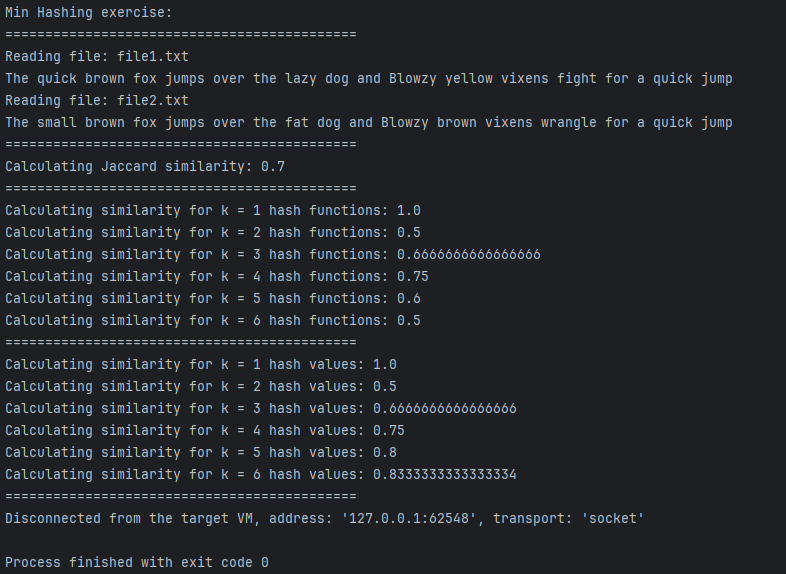
\includegraphics[scale = 0.4]{MinHashOutput.PNG}
\end{figure}

\question[1]{Quadtrees}

\begin{enumerate}
\item Give 8 points, with coordinates where each dimension has values in the range $[0,100]$, and sort them into two insertion orders.
The first should have less empty leaf nodes if inserted into a quadtree than if they were inserted into a PR quadtree.
The second one the other way around.

Submit the points, the two insertion orders and draw the (PR) quadtrees. You can either draw them as tree or as the grid visualization.

{\bf Solution:}\\
The quadtree has less empty leave nodes than the pr-quadtree if the 8 points get inserted in the following order:
$A(30,40); B(20, 75); C(78,75); D(10,10); E(80, 30); F(60, 5); G(90, 2); H(70, 35)$\\\\
Quadtree:\\
  \begin{tikzpicture}[level distance=1.5cm,
  level 1/.style={sibling distance=3cm},
  level 2/.style={sibling distance=3cm},
  level 3/.style={sibling distance=3cm},
  level 4/.style={sibling distance=3cm},
  level 5/.style={sibling distance=3cm},
  level 6/.style={sibling distance=3cm}]
  \node[draw]{$30,40$}
    child{node[draw]{20,75}}
    child{node[draw]{78,75}}
    child{node[draw]{10,10}}
    child{
      node[draw]{80,30}
      child{node[draw]{70,35}}
      child{node[draw]{60,5}}
      child{node[draw]{90,2}}
      child{node[draw]{null}}
    };
  \end{tikzpicture}

PR-Quadtree:\\
\begin{tikzpicture}[level distance=1.5cm,
  level 1/.style={sibling distance=5cm},
  level 2/.style={sibling distance=1cm},
  level 3/.style={sibling distance=1.5cm}]
  \node[draw]{$A$}
    child{node[draw]{20,75}}
    child{node[draw]{78,75}}
    child{
      node[draw]{B}
      child{node[draw]{null}}
      child{node[draw]{30,40}}
      child{node[draw]{10,10}}
      child{node[draw]{null}}
      }
    child{
      node[draw]{C}
      child{node[draw]{70,35}}
      child{node[draw]{80,30}}
      child{node[draw]{60,5}}
      child{node[draw]{90,2}}};
  \end{tikzpicture}

  Changed order:
  
  $G(90, 2); D(10,10); A(30,40); F(60, 5); B(20, 75); C(78,75); E(80, 30); H(70, 35)$\\\\
  Quadtree:\\
  \begin{tikzpicture}[level distance=1.5cm,
    level 1/.style={sibling distance=3cm},
    level 2/.style={sibling distance=3cm},
    level 3/.style={sibling distance=3cm},
    level 4/.style={sibling distance=3cm},
    level 5/.style={sibling distance=3cm},
    level 6/.style={sibling distance=3cm}]
    \node[draw]{$90, 2$}
      child{
        node[draw]{10,10}
        child{node[draw]{null}}
        child{
          node[draw]{30,40}
            child{node[draw]{20,75}}
            child{node[draw]{78, 75}}
            child{
              node[draw]{80, 30}
              child{node[draw]{70, 35}}
              child{node[draw]{null}}
              child{node[draw]{null}}
              child{node[draw]{null}}}
            }
        child{node[draw]{60, 5}}
        child{node[draw]{null}}
      }
      child{node[draw]{null}}
      child{node[draw]{null}}
      child{node[draw]{null}};
  
    \end{tikzpicture}

    PR-Quadtree:
    The PR-Quadtree is not relying on the order of the tree items. No mater what order is used the tree will be always the same. 
  
\item
Assuming we have the whole dataset present upon insertion, describe one possible way that optimizes the creation of the quadtree, such that the height of the resulting quadtree is minimized.
Note that before the bulk-loading, preprocessing of the data is allowed.

{\bf Solution: }
The data point that has the is the closesd to the average of the y koordinate and the x koordinate should be choosen to inserted first. From than on this gets repreated for each sub quadrant. until all the data is put into the tree structure.

\item
  Assuming we are given uniformly distributed point data, what is the probability that a node at depth $k$ contains a particular point in a PR Quad tree? 
  Additionally, for a collection of $v$ points, calculate the probability that none of the points lies in a given cell at depth $k$? 

{\bf Solution: }
The probability is $1/4^{k}$ for a particular point.\\
The probability that no point is inside a specific cell at the depth k is $(1-1/4^k)$

\end{enumerate}

\newpage
\question[1]{kd tree}

\begin{enumerate}
\item
  Insert the following values, in provided order, into an empty $k$d tree, with $k=3$:

  \begin{minipage}{0.48\textwidth}
    \begin{enumerate}[label={\color{gray}\arabic*.}]
      \item (19, 31, 83)
      \item (64, 27, 97)
      \item (66, 8, 101)
      \item (99, 86, 34)
      \item (12, 92, 55)
      \item (76, 39, 85)
    \end{enumerate}
  \end{minipage}
  \begin{minipage}{0.48\textwidth}
    \begin{enumerate}[label={\color{gray}\arabic*.}]
      \setcounter{enumii}{6}
      \item (85, 68, 4)
      \item (98, 60, 59)
      \item (13, 52, 9)
      \item (44, 39, 91)
      \item (29, 35, 57)
      \item (43, 15, 98)
    \end{enumerate}
  \end{minipage}

  Draw the result as a tree, like shown in the lecture.
  Note which values you used for the split.

{\bf Solution:}\\\\
\textbf{KD Tree implementation}

\begin{tikzpicture}
[
squarednode/.style={rectangle, draw=blue!60, fill=green!5, very thick, minimum size=5mm},
]

%Nodes
\node[squarednode]      (maintopic)                 {\textbf{1:} 19, 31, 83};
\node[squarednode]      (leftchild)       [below left=of maintopic] {\textbf{5:} 12,92,55} ;   
\node[squarednode]      (rightchild)      [below right=of maintopic] {\textbf{2:} 64,27,97};
\node[squarednode]      (leftchild-L)      [below left=of leftchild] {\textbf{9:} 13,52,9} ; 
\node[squarednode]      (R-LeftChild)     [below left=of rightchild] {\textbf{3: }66,8,101};
\node[squarednode]      (R-RightChild)    [below right=of rightchild] {\textbf{4:} 99,86,34};
\node[squarednode]      (R-LeftChild-L)   [below left = of R-LeftChild] {\textbf{12:} 43,15,98};
\node[squarednode]     (R-RightChild-L)    [below left = of R-RightChild] {\textbf{7:} 85,68,4};
\node[squarednode]     (R-RightChild-R)    [below right = of R-RightChild] {\textbf{6:} 76,39,85};
\node[squarednode]     (R-RightChild-R-L)  [below left = of R-RightChild-R] {\textbf{10:} 44,39,91};
\node[squarednode]     (R-RightChild-R-R) [below = of R-RightChild-R] {\textbf{8:} 98,60,59};
\node[squarednode]     (R-RightChild-R-L-L) [below left = of R-RightChild-R-L] {\textbf{11: }29,35,57};


%Lines
\draw[->]  (maintopic) -- (leftchild);
\draw[->]  (leftchild) -- (leftchild-L);
\draw[->]  (maintopic) -- (rightchild);
\draw[->]  (rightchild) -- (R-LeftChild);
\draw[->]  (rightchild) -- (R-RightChild);
\draw[->]   (R-RightChild) -- (R-RightChild-R);
\draw[->]   (R-RightChild) --(R-RightChild-L);
\draw[->] (R-RightChild-R) -- (R-RightChild-R-L);
\draw[->] (R-RightChild-R) -- (R-RightChild-R-R);
\draw[->] (R-RightChild-R-L) -- (R-RightChild-R-L-L);
\draw[->] (R-LeftChild) -- (R-LeftChild-L);

\end{tikzpicture}

\begin{tabular}{ |c|c|c| } 
 \hline
 Data Points & Split Value & Split Position \\ [0.5ex] 
 \hline\hline
 \hline
  (19, 31, 83) & 19 & 0 \\ 
 (64, 27, 97) & 64 & 0\\ 
 (66, 8, 101) & 8 & 1 \\ 
 (99, 86, 34) & 86 & 1 \\ 
 (12, 92, 55) & 12 & 0 \\ 
 (76, 39, 85) & 85 & 2\\ 
 (85, 68, 4) & 4 & 2 \\ 
 (98, 60, 59) & 98 & 0 \\ 
 (13, 52, 9) & 52 & 1 \\ 
 (44, 39, 91) & 44 & 0\\ 
 (29, 35, 57) & 35 & 1\\ 
 (43, 15, 98) & 98 & 2 \\ 
 \hline
\end{tabular}
\\
\newline
\newline
In the above table, we are considering the given data points/ co-ordinates as (X,Y,Z) and (0,1,2) to represent the split positions for the respective X,Y,Z values
\\



\item
Adaptive kd tree

Provide \textbf{in detail} an algorithm, in pseudo code, that takes a list of coordinates in $k$ dimensions and builds a $k$d tree.
This tree may have a maximum of ten data points in its leaves.
The dimension used for the split should be the one with the largest variance.
The value used for the split, should be the average of the split dimension of all relevant coordinates.

{\bf Solution:}
The Adaptive kd tree is the variant of KD Tree, where the partitioning is done not only 		on the basis of alternating dimensions, but also depends on data distribution. 
Not sure of the algorithm 


\end{enumerate}

\end{document}
